\documentclass[11pt]{article}
\usepackage[margin=1in]{geometry}
\usepackage{amsmath,amssymb}
\usepackage{booktabs}
\usepackage{array}
\usepackage{graphicx}
\usepackage{xcolor}
\usepackage[hidelinks]{hyperref}
\usepackage{enumitem}
\setlength{\parskip}{4pt}
\newcommand{\lod}{\mathrm{LOD}}
\newcommand{\KL}{\mathrm{KL}}
\newcommand{\code}[1]{\texttt{#1}}
\title{GARLIC's automatic LOD cutoff:\\ the sign-anchored mode rule, and how it differs from the valley rule it replaces}
\author{GARLIC \code{low-cov} branch, commits \code{525bf13}, \code{f7bc79f}}
\date{October 2026}
\begin{document}
\maketitle

\begin{abstract}
GARLIC calls runs of homozygosity by thresholding window LOD scores, and by default it chooses the threshold itself from the density of LOD scores across the cohort. Both the previous rule and the new one place the threshold at the \emph{valley} of that density between its two modes; the two rules differ in how the two modes are identified and in what happens when the density does not have two. The new rule identifies the modes by \emph{sign}: the non-autozygous mode is the dominant peak at $\lod<0$, the autozygous mode the dominant peak at $\lod>0$, because the expected LOD of a window is negative in one state and positive in the other at any depth. The previous rule took the two most ``persistent'' maxima of a smoothed density, with no reference to sign, no minimum height, and a fallback to 0 when the valley lay far from zero. On every density where the previous rule was sound, the new one returns the identical cutoff: 26 of the 40 benchmark cohorts, including the genome-wide bundled example, agree to machine precision, of the 14 that differ, 13 are cases where the previous rule placed the cutoff inside the non-autozygous component, on a tail bump, or at its fallback of 0, and in one (hard genotype calls at 4$\times$ in a low-diversity population) its cutoff happened to be useful and the new rule declines (\S\ref{sec:validation}). Where it was not, the previous rule placed the cutoff inside the non-autozygous component (chromosome 21 of the bundled example: cutoff $-55.7$, 22 Mb of ROH per individual on a 47 Mb chromosome; now $-0.33$ and 3.6 Mb) or on a density-$10^{-4}$ tail bump (a simulated Ne 2\,000 cohort at 2$\times$: cutoff $-57.8$, $F_{\rm ROH}=0.997$). Densities with no autozygous mode now end the run with no calls and a warning rather than with an invented threshold. Rebuilt and re-run on all 47 automatic-cutoff arms of the benchmark, the compiled rule reproduces these predictions exactly. The hard-call arms that the new rule declines at 1--2$\times$ are recovered once the genotypes are the maximum-likelihood calls from PL rather than bcftools' prior-based calls (\S\ref{sec:validation}).
\end{abstract}

\section{What both rules share}

For each individual, GARLIC slides a window of $w$ SNPs along each chromosome and sums per-site log-likelihood ratios of the autozygous (A) against the non-autozygous (N) emission model,
\[
\lod_{\rm win} = \sum_{i\in \rm win} \log_{10}\frac{P(\text{data}_i\mid A)}{P(\text{data}_i\mid N)},
\]
where $\text{data}_i$ is a called genotype (\code{--tped}, \code{--vcf}) or a genotype-likelihood triplet (\code{--gl-beagle}, \code{--gl-type PL}). Windows in autozygous stretches have high LOD, windows elsewhere low LOD, and the pooled density of window LODs across the cohort is a two-component mixture. GARLIC estimates that density by a Gaussian kernel density estimate (nrd0 bandwidth, 512 grid points, written to \code{<out>.<w>SNPs.kde}) and places the cutoff at the \emph{density minimum between the two modes}. Windows above the cutoff are assembled into runs; the run-length classes (\code{--size-bounds}) are applied afterwards.

This document is about one step only: given the density on its grid, which two points are ``the modes''.

\section{Why the two modes lie on opposite sides of zero}
\label{sec:sign}

Let $P_N(g\mid p)$ and $P_A(g\mid p)$ be the emission probabilities of a called genotype $g$ at a site of alternate-allele frequency $p$ (for the autozygous state $P_A$ puts mass $\varepsilon\cdot 2pq$ on the heterozygote and the rest on the two homozygotes in proportion to allele frequency). If the genotype at a site that is truly non-autozygous is drawn from $P_N$, the expected per-site LOD is
\[
\mathbb{E}_N[\ell] = \sum_g P_N(g)\log_{10}\frac{P_A(g)}{P_N(g)} = -\frac{\KL(P_N\,\|\,P_A)}{\ln 10} \le 0,
\]
and at a truly autozygous site $\mathbb{E}_A[\ell] = +\KL(P_A\,\|\,P_N)/\ln 10 \ge 0$, with equality only if the two emission distributions coincide (Gibbs' inequality). A window LOD is a sum over $w$ sites, so the centre of the non-autozygous mode is $-\frac{1}{\ln 10}\sum_i \KL(P_N\|P_A)_i<0$ and the centre of the autozygous mode is $+\frac{1}{\ln 10}\sum_i\KL(P_A\|P_N)_i>0$.

With genotype likelihoods the per-site LOD is a ratio of \emph{marginal} likelihoods of the reads, $\log_{10} m_A(r)/m_N(r)$ with $m_S(r)=\sum_g P_S(g)L(r\mid g)$, and under state $S$ the reads are distributed as $m_S$; the same inequality gives $\mathbb{E}_N[\ell]\le 0\le \mathbb{E}_A[\ell]$. As depth falls, $L(r\mid g)$ flattens, $m_A\to m_N$, and both expectations shrink toward zero: the two modes \emph{merge} (benchmark: $-3.9/{+1.5}$ at 1$\times$, $-25/{+5.8}$ at 4$\times$, $-55/{+9.6}$ on true genotypes), but neither changes sign. Three consequences fix the design:
\begin{enumerate}[nosep]
\item The non-autozygous mode is \emph{always} below zero and the autozygous mode \emph{always} above it, at any depth, error rate, window size or allele-frequency spectrum, as long as the data are generated by the emission model GARLIC evaluates.
\item The two divergences are very unequal (a heterozygote is nearly impossible under A, so $\KL(P_N\|P_A)\gg\KL(P_A\|P_N)$: for $p=0.3$, $\varepsilon=10^{-3}$, about 2.6 vs 0.6 nats per site). The non-autozygous mode therefore sits far from zero ($-46$ predicted for a 60-site window averaged over a neutral frequency spectrum; $-61$ observed) and the autozygous mode close to it ($+12$ predicted, $+8$ observed). This is why the valley, and hence the automatic cutoff, is normally \emph{negative}.
\item Loss of signal appears as a \emph{unimodal} density, never as two modes on the same side of zero. Two peaks on the same side are two bumps of one component.
\end{enumerate}
The anchor fails only when the data violate the model. The one case found in practice is hard genotype calls made under a population prior at low depth. \code{bcftools call -m} multiplies each sample's genotype likelihoods by a prior derived from the cohort's allele frequency; with one or two reads the likelihoods barely separate a homozygote from a heterozygote, so the prior decides, and at intermediate frequency it decides ``heterozygous''. In the benchmark's 1$\times$ calls 70\% of heterozygote calls are of this kind (the sample's own PL favours a homozygote; most come from single-read samples, which cannot show a heterozygote at all), 44\% at 2$\times$, 14\% at 4$\times$ and 1\% at 8$\times$. Inside a run each such call costs a $\log_{10}\varepsilon$-scale penalty, and at 1--2$\times$ the autozygous mode moves below zero (samples with no reads at all are written as missing and are not the problem). This is a pipeline defect, not a mode-finding one: use the maximum-likelihood genotype from PL (\code{bench/scripts/ml\_genotypes.py}), or give GARLIC the likelihoods themselves (\code{--gl-type PL}, \code{--gl-beagle}).

\section{The previous rule}
\label{sec:old}

\code{get\_min\_btw\_modes} slid a window of $s=20$ grid points over the 512-point density, recorded each windowed arg-max and the number of consecutive windows for which it remained the maximum (its ``persistence''), took the \emph{two most persistent} maxima as the modes, and returned the density minimum between them. If the resulting valley lay more than one LOD per SNP from zero ($|{\rm valley}|\ge w$) it was discarded and 0 applied instead.

The rule has three structural weaknesses, each observed on real or simulated data (Fig.~\ref{fig:modes}, Table~\ref{tab:cases}):
\begin{enumerate}[nosep]
\item \textbf{Persistence saturates.} Any bump broader than $s$ grid points ($\approx 8$ LOD on a 200-LOD grid) persists for exactly $s$ windows, so on most densities two to four maxima tie at the maximum count, and the tie is broken by height. Height carries no information about which component a bump belongs to.
\item \textbf{No height floor.} A bump of density $10^{-4}$ in the far tail qualifies as a mode as readily as the main peak.
\item \textbf{No sign constraint.} Nothing prevents both chosen maxima from lying in the non-autozygous component, which happens whenever that component is lumpy (many windows, small bandwidth, a low-diversity population) or the autozygous mode is absent or merged (very low depth, hard calls at 1--2$\times$, depths pooled across strata). The valley between two bumps of the same component is then reported as the cutoff, and typically calls a large part of the genome. The $|{\rm valley}|\ge w\to 0$ guard caught only the most extreme instances, and 0 is itself an arbitrary threshold.
\end{enumerate}

\section{The new rule}
\label{sec:new}

\code{identifyLODModes} (\code{garlic-kde.cpp}) takes the density $(x_j,y_j)$ on its grid and proceeds as follows.
\begin{enumerate}[nosep]
\item \textbf{Candidate peaks.} A grid point is a candidate if it is an interior local maximum, its density is at least $2\%$ of the maximum density, and it holds the windowed maximum for at least $s/2=10$ of the $s$-point windows that contain it. The persistence walk is the same one the old rule used; it is now a \emph{smoothness filter} that removes ripples on the flank of a broad bump, and nothing more.
\item \textbf{Modes by sign.} The non-autozygous mode $m_N$ is the tallest candidate with $x<0$; the autozygous mode $m_A$ is the tallest candidate with $x>0$. (A candidate exactly at 0 belongs to neither.)
\item \textbf{Cutoff.} If both exist the density is \emph{bimodal} and the cutoff is $\arg\min_{m_N\le x\le m_A} y$, the valley between them, exactly as before.
\item \textbf{Verdicts.} If only $m_N$ exists the density is \emph{unimodal-null}: the windows show no resolvable autozygous excess. The run completes---all per-individual reports are written---with no ROH calls, a warning on \code{stderr} that names the likely causes (depth or sites per window too low for these samples; hard genotype calls with prior-imputed no-read genotypes; individuals of very different depth pooled, see \code{--stratify-cutoff}) and the flags that address them, and \code{params.json} records \code{"lod\_cutoff": null}, \code{"lod\_density\_verdict":} \code{"unimodal-null"} and the location of the mode that was found. If only $m_A$ exists (\emph{unimodal-autozygous}) the non-autozygous state is not represented---an all-autozygous sample, or an input that does not mean what the model assumes (posteriors instead of likelihoods, frequencies from the wrong population)---and GARLIC stops with a message asking for \code{--lod-cutoff}. The $\pm w$ guard is removed: a valley is defined by the two modes it lies between, not by its distance from zero.
\item \textbf{Reporting.} Every automatic run logs ``LOD score modes: non-autozygous at $m_N$, autozygous at $m_A$; valley between them at $c$'' and writes the three numbers and the verdict to \code{params.json}, so a reader can see what was identified, not just what was applied.
\end{enumerate}

\paragraph{Per-individual modes (\code{--stratify-cutoff}).} Each individual's non-autozygous mode, used to group individuals into evidence strata, was ``the lowest peak at least 25\% as tall as the tallest peak'' of a smooth (2$\times$nrd0) density of that individual's windows. For an individual with $F\approx0.5$ the broad null peak is 0.245$\times$ the height of the narrow autozygous peak, so the rule took the \emph{autozygous} mode as the null (in all nine resolvable benchmark cohorts). It is now the lowest local maximum at $\lod<0$ that is at least 10\% as tall as the tallest \emph{negative} maximum. An individual with no negative peak at all (its two components have merged, as happens for inbred individuals at 1$\times$) is ``unresolved'' and takes the largest stratum's cutoff, labelled \code{pooled\_unresolved\_mode} in \code{<out>.ind.tsv}; previously it silently received a positive ``null'' mode. Strata valleys use \code{identifyLODModes}; a cohort in which every stratum is unimodal-null receives the no-call outcome above.

\section{Precisely how the two rules differ}
\label{sec:diff}

Both rules are \emph{valley rules}: given two modes, both return the density minimum between them, and the minimum is computed identically. The differences are entirely in the identification step and in the handling of its failure:

\begin{center}\small
\begin{tabular}{p{0.28\textwidth}p{0.31\textwidth}p{0.31\textwidth}}
\toprule
 & previous rule & new rule \\
\midrule
what defines a mode & one of the two most persistent windowed maxima (ties broken by height) & a local maximum $\ge 2\%$ of the peak density, persisting $\ge s/2$ windows \\
how the two are told apart & they are not: ``left'' and ``right'' of whatever two were chosen & by sign: dominant peak below 0 is N, dominant peak above 0 is A \\
two peaks on one side of zero & taken as the two modes; valley between them applied & the taller is that side's mode; the other side is searched separately \\
tail bump of negligible density & eligible & excluded by the height floor \\
valley far from zero & replaced by 0 (silently before \code{perf-fixes}, with a warning since) & no rule; the valley is wherever the two modes put it \\
no peak above 0 & valley between two null bumps, or 0 & \emph{unimodal-null}: no calls, warning, \code{null} in \code{params.json} \\
no peak below 0 & valley between two autozygous bumps & \emph{unimodal-autozygous}: stop, ask for \code{--lod-cutoff} \\
what is reported & the cutoff & the cutoff, both modes and the verdict \\
per-individual mode & lowest peak $\ge 25\%$ of the tallest peak & lowest negative peak $\ge 10\%$ of the tallest negative peak; \emph{unresolved} if none \\
\bottomrule
\end{tabular}
\end{center}

When a density has one clear peak below zero and one above, the old rule's two most persistent maxima \emph{are} those two peaks, the valley is the same grid point, and the cutoff is identical to the last digit. This is the situation on every benchmark cohort with adequate signal (pedigree cohorts at $\ge1\times$ with likelihoods, hard calls at $\ge4\times$, HGDP array data genome-wide, the bottleneck population at every depth), and existing results on such data do not change. Table~\ref{tab:cases} lists the cases where they do.

\begin{table}[h]\centering\footnotesize
\caption{Cohorts of the benchmark test bed on which the two rules differ (GARLIC's own density grids). Where both rules agree (26 of 40 cohorts) the cutoffs are identical to machine precision.}
\label{tab:cases}
\begin{tabular}{p{0.25\textwidth}p{0.1\textwidth}rrp{0.27\textwidth}}
\toprule
cohort & data & previous & new & why they differ \\
\midrule
bundled example, chr21 only & array genotypes, 45 ind. & $-55.7$ & $-0.33$ & two bumps of the null component ($-62.7$, $-51.5$) \\
bundled example, mixed depths, chr21 & GL, pooled & $-17.8$ & none (unimodal-null) & both chosen modes negative ($-29$, $-6$) \\
bundled example, mixed depths, genome & GL, pooled & 0 (guard) & $+1.13$ & valley between two null bumps ($-143$, $-13.5$) discarded by the guard \\
Ne 2\,000 population, true genotypes & calls & $-48.3$ & $-0.83$ & lumpy null component ($-53.9$, $-43.6$) \\
Ne 2\,000 population, 2$\times$ & GL & $-57.8$ & $+0.99$ & tail bump, density $10^{-4}$, at $-61$ \\
Ne 2\,000 population, 1$\times$ & GL & $-5.6$ & none (unimodal-null) & two null bumps ($-6.7$, $-4.2$) \\
Ne 2\,000 population, 4$\times$ & hard calls & $-7.0$ & none (unimodal-null) & autozygous peak pushed to $-3.9$ by prior-driven het calls; here the old cutoff was useful \\
no-run smoke cohort, 1$\times$ & GL & $-10.4$ & $-0.55$ & two null bumps ($-12.6$, $-8.4$) \\
pedigree, bottleneck, Ne 2\,000 at 1--2$\times$ & hard calls & 0 (guard) & none (unimodal-null) & prior-driven heterozygote calls (\S\ref{sec:sign}) \\
\bottomrule
\end{tabular}
\end{table}

\section{Evidence}

\paragraph{Reproduction.} A line-by-line port of the previous rule applied to GARLIC's own \code{.kde} grids reproduces GARLIC's chosen cutoff on all 40 benchmark cohorts to $<0.01$ LOD, so the comparison above is of the code as it ran.

\paragraph{Stability.} Resampling individuals with replacement (10 replicates), the two rules have identical bootstrap standard deviations of the cutoff wherever both are sound (0.07 LOD at 1$\times$, 0.28 at 4$\times$, 1.7 on true genotypes, 0.35 on HGDP array data, 0.8--1.0 on the population cohorts). Where they differ the old rule scatters (SD 6.7 on the mixed-depth fixture, 15 on 2$\times$ hard calls, with the guard firing in 6 of 10 replicates) and the new one is stable (0.8) or consistently reports unimodal-null (10 of 10). A two-component mixture fit was also evaluated and rejected: it trades recall for precision and is unstable with heavy tails.

\paragraph{Accuracy.} Against window labels from the simulated truth, the valley is on the conservative side of the truth-optimal threshold in every pedigree cohort (the Youden cutoff lies below it, by about 1 LOD at 1$\times$ and 7 LOD at 8$\times$), and segment-level recall of runs $\ge1$ Mb is 0.98--0.99 wherever the modes are correctly identified. On the Ne 2\,000 cohort, re-running GARLIC at the new cutoffs brings the arms that had failed (true genotypes, 2$\times$) to the same size-stratified precision and recall as the arms where the old rule happened to work (precision 0.90 for runs $>1$ Mb, 0.70--0.76 for 0.5--1 Mb; recall of IBD tracts with TMRCA $\le 1000$ generations 0.86--0.92 for $\ge 0.5$ Mb), down from 29--130 Mb of ``ROH'' $>1$ Mb per individual.

\paragraph{What a genome without long runs looks like.} A control cohort with no IBD tract longer than 1 Mb by construction still shows a small positive mode (5\% of the peak density) from short background IBD, and both rules place the cutoff at $+4.9$; GARLIC emits only class-A calls (longest 261 kb, 1.2\% of the genome). The unimodal-null verdict is therefore a statement about data quality, not about the absence of ROH, and the warning says so.

\begin{figure}[p]\centering
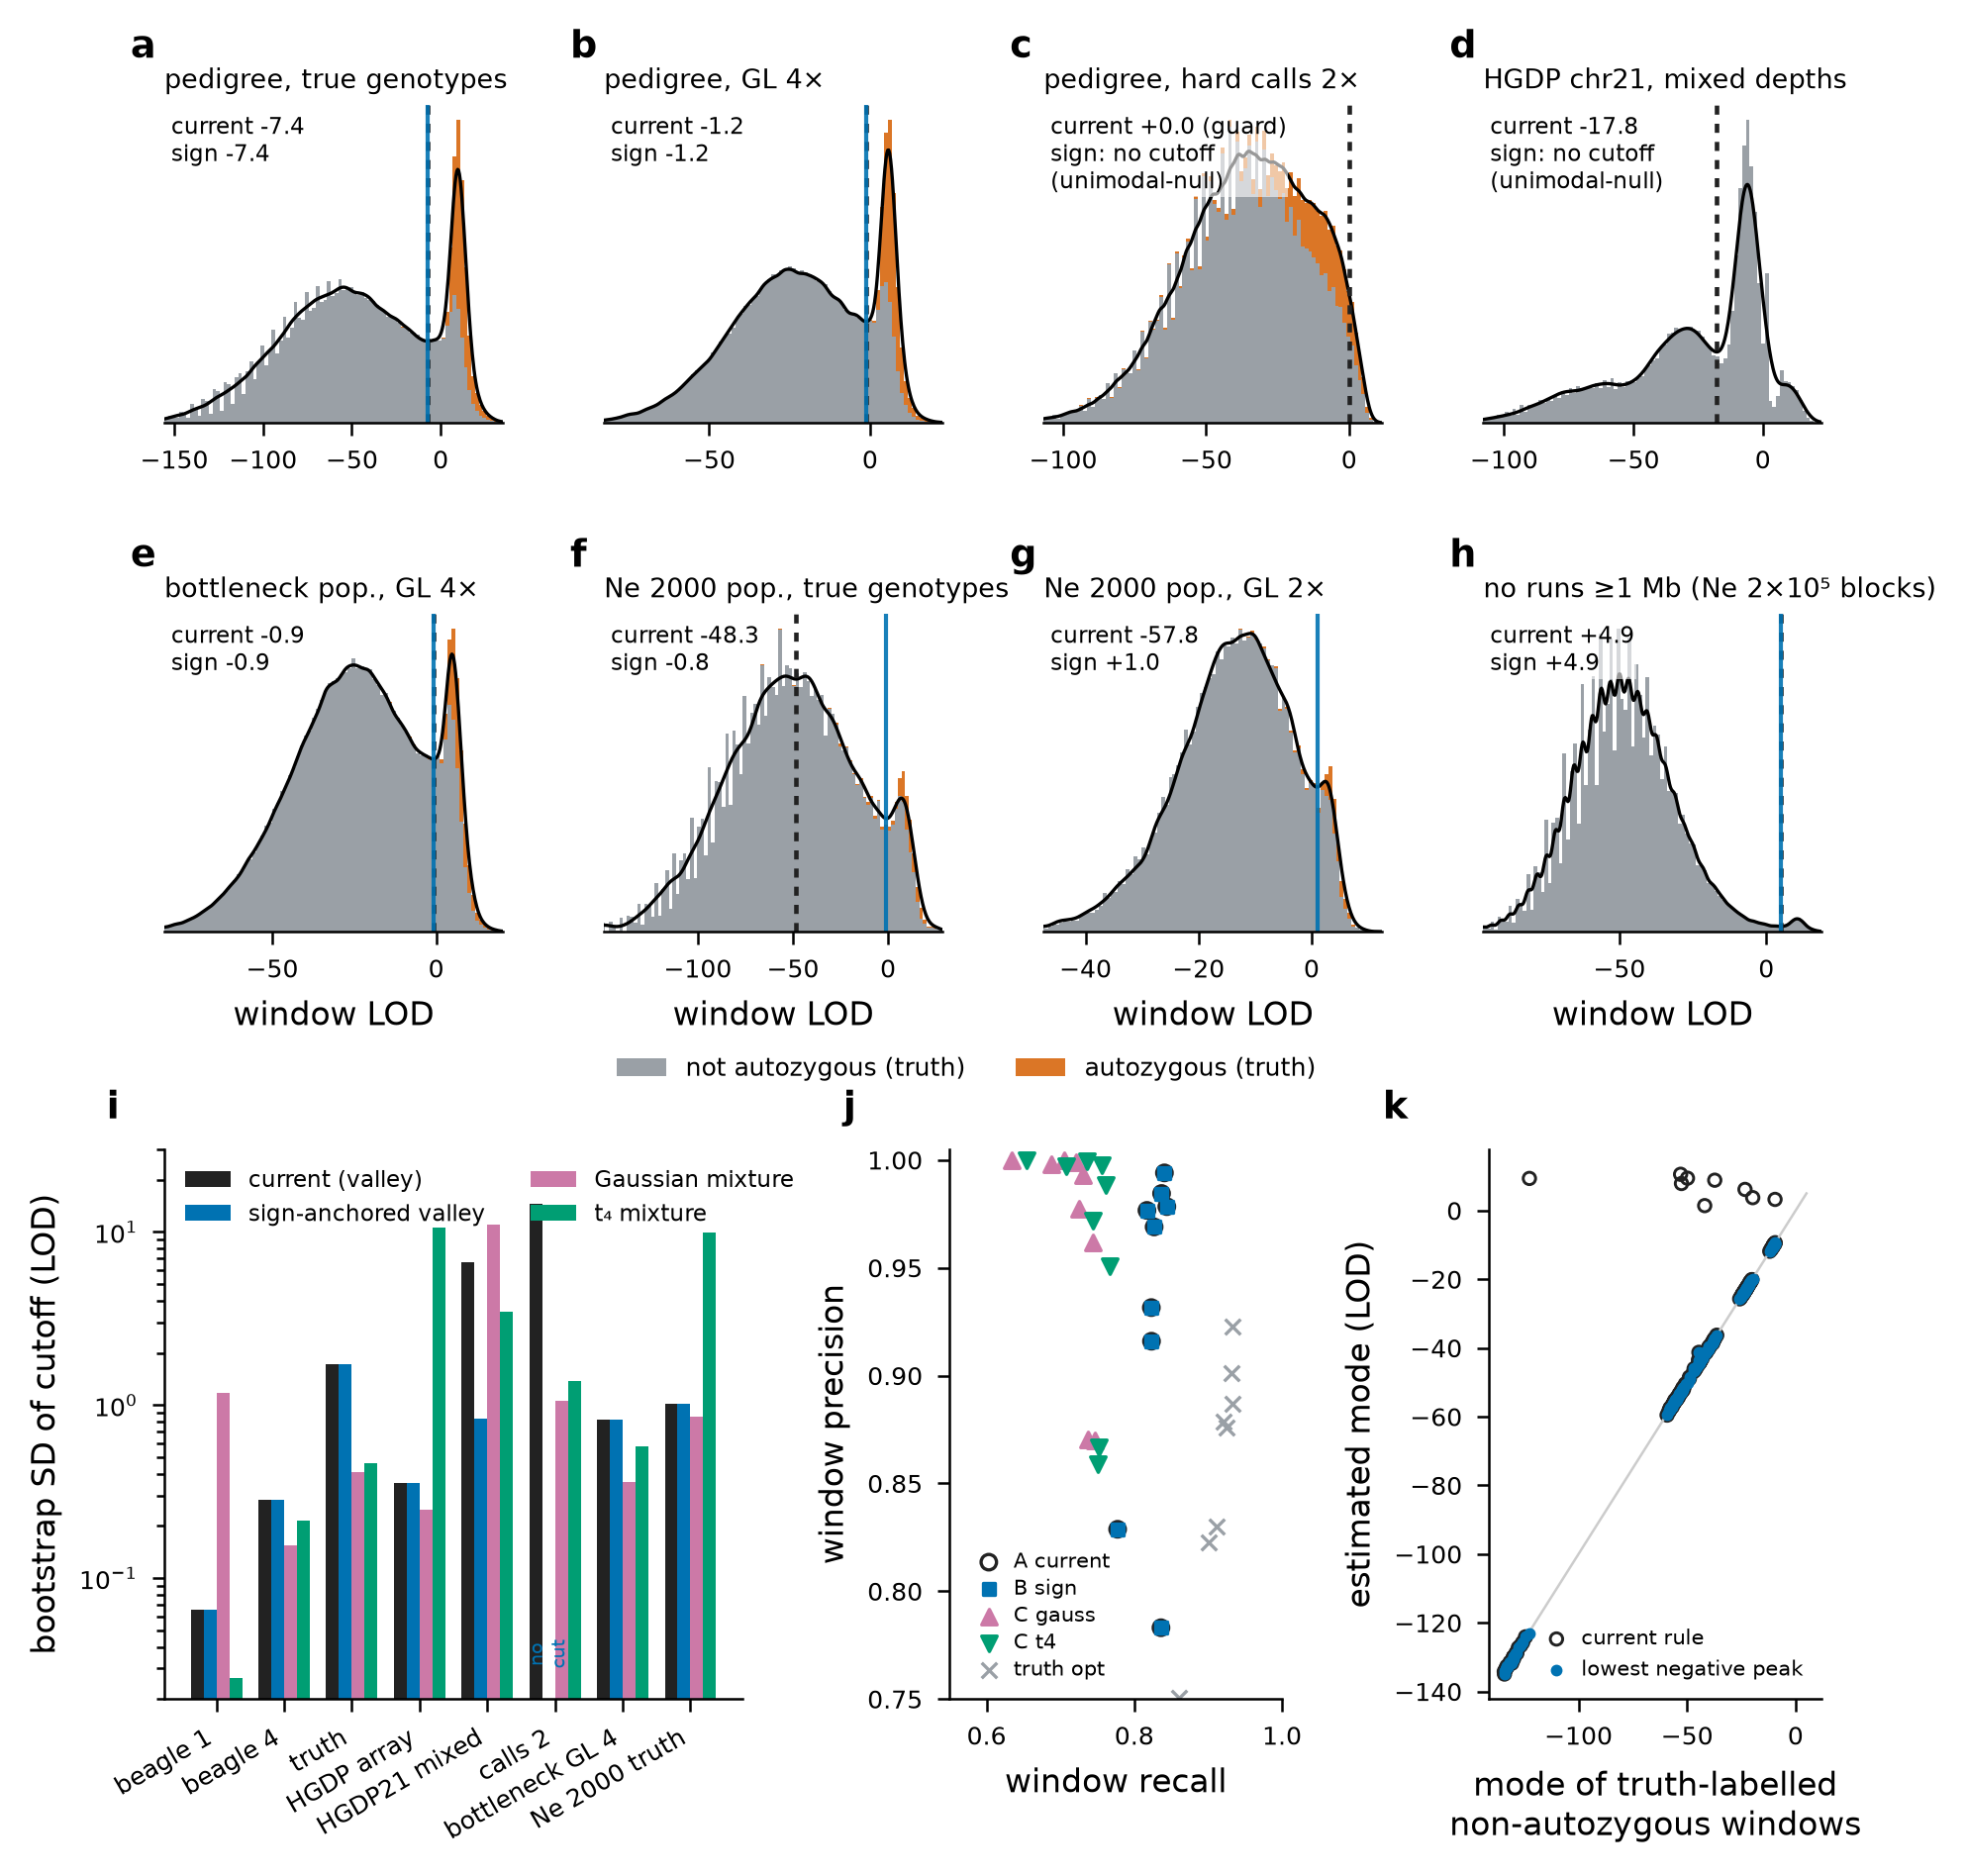
\includegraphics[width=\textwidth]{lod-modes-study.png}
\caption{Window-LOD densities on GARLIC's own grids with the previous (dashed) and new (solid blue) cutoffs: (a--c) pedigree cohort on true genotypes, 4$\times$ likelihoods and 2$\times$ hard calls; (d) bundled chr21 fixture at mixed depths; (e) bottleneck population; (f, g) Ne 2\,000 population on true genotypes and at 2$\times$; (h) no-run control. Orange: windows inside true autozygous segments. (i) Bootstrap SD of the cutoff over resampled individuals. (j) Window precision and recall at each rule's cutoff on the pedigree cohorts. (k) Per-individual non-autozygous mode, previous rule (open) and new rule (filled), against the mode of truth-labelled non-autozygous windows.}
\label{fig:modes}
\end{figure}


\section{End-to-end validation on the benchmark}
\label{sec:validation}

GARLIC was rebuilt with the new rule and every automatic-cutoff arm of the benchmark was re-run from its stored inputs: the pedigree cohort (21 arms: true genotypes; ANGSD likelihoods at 1, 2, 4, 8$\times$ with three error rates; bcftools PL and hard calls at 1--8$\times$), the bottleneck population and the Ne 2\,000 population (13 arms each). The compiled rule reproduces the Python prototype on every arm. In 36 of the 47 the cutoff is identical to the previous one, and so are the calls and every score: pedigree 19 of 21, bottleneck 11 of 13, Ne 2\,000 6 of 13. Table~\ref{tab:validation} lists the 11 that change, scored against the simulated truth by run-length class. For the pedigree, precision is against the attainable set (pedigree autozygosity plus background runs called on true genotypes) and recall against pedigree autozygosity. For the population cohorts, precision is the fraction of called bases inside within-individual IBD tracts $\ge$100 kb, and recall is against tracts with TMRCA $\le$1000 generations.

\begin{table}[h]\centering\footnotesize
\caption{The benchmark arms whose cutoff changes, scored on runs $>$1 Mb as precision / recall / Mb called per individual (``no calls'': the run completed with the unimodal-null verdict). The last column re-runs the hard-call arms with the maximum-likelihood genotype from PL in place of bcftools' prior-based call.}
\label{tab:validation}
\setlength{\tabcolsep}{4pt}
\begin{tabular}{>{\raggedright\arraybackslash}p{0.085\textwidth}>{\raggedright\arraybackslash}p{0.12\textwidth}rr>{\raggedright\arraybackslash}p{0.17\textwidth}>{\raggedright\arraybackslash}p{0.14\textwidth}>{\raggedright\arraybackslash}p{0.15\textwidth}}
\toprule
cohort & data & previous & new & previous rule & new rule & new rule, \\
 & & cutoff & cutoff & & & ML genotypes \\
\midrule
pedigree & hard calls 1$\times$ & $0$ & none & -- / 0.04 / 0.0 & no calls & 1.00 / 1.00 / 14.6 \\
pedigree & hard calls 2$\times$ & $0$ & none & -- / 0.15 / 0.0 & no calls & 1.00 / 1.00 / 14.7 \\
bottleneck & hard calls 1$\times$ & $0$ & none & -- / 0.06 / 0.0 & no calls & 0.95 / 1.00 / 4.1 \\
bottleneck & hard calls 2$\times$ & $0$ & none & -- / 0.21 / 0.0 & no calls & 0.96 / 1.00 / 4.1 \\
Ne 2\,000 & true geno\-types & $-48.32$ & $-0.83$ & 0.38 / 1.00 / 29.0 & 0.90 / 0.86 / 3.1 & n/a \\
Ne 2\,000 & GL 2$\times$ & $-57.85$ & $+0.99$ & 0.20 / 1.00 / 130.0 & 0.90 / 0.90 / 3.1 & n/a \\
Ne 2\,000 & GL 1$\times$ & $-5.61$ & none & 0.28 / 1.00 / 49.1 & no calls & n/a \\
Ne 2\,000 & PL 1$\times$ & $-54.69$ & none & 0.20 / 1.00 / 130.0 & no calls & n/a \\
Ne 2\,000 & hard calls 1$\times$ & $0$ & none & -- / 0.00 / 0.0 & no calls & no calls \\
Ne 2\,000 & hard calls 2$\times$ & $0$ & none & -- / 0.07 / 0.0 & no calls & no calls \\
Ne 2\,000 & hard calls 4$\times$ & $-6.99$ & none & 0.90 / 0.83 / 2.7 & no calls & 0.90 / 0.86 / 3.1 \\
\bottomrule
\end{tabular}
\end{table}

Three groups of changes:
\begin{enumerate}[nosep]
\item \textbf{Cutoffs inside the non-autozygous component, now corrected} (Ne 2\,000 true genotypes and GL 2$\times$). The previous rule called 29 and 130 Mb of ``runs $>$1 Mb'' per individual at precision 0.38 and 0.20; the new rule calls 3.1 Mb at precision 0.90 with recall 0.86--0.90, the same as the arms where the previous rule happened to work.
\item \textbf{Cutoffs on noise, now declined} (Ne 2\,000 GL 1$\times$ and PL 1$\times$, previous cutoffs $-5.6$ and $-54.7$, 49--130 Mb per individual at precision 0.20--0.28; hard calls at 1--2$\times$ in all three cohorts, previous fallback 0 with recall $\le$0.21). These now complete with no calls and the unimodal-null warning.
\item \textbf{One useful cutoff lost} (Ne 2\,000 hard calls at 4$\times$). The previous rule's two ``modes'' were the null peak at $-42.3$ and an autozygous peak displaced to $-3.9$ by prior-driven heterozygote calls, and its valley at $-7.0$ gave precision 0.90 and recall 0.83. The new rule reads a density with no peak above zero and declines. This is the cost of refusing to treat two peaks on the same side of zero as the two modes. On the data the model describes the refusal is correct, but here the cause is the genotype caller. With maximum-likelihood genotypes the density becomes bimodal again and the arm returns to precision 0.90, recall 0.86.
\end{enumerate}
Maximum-likelihood genotypes also recover the hard-call arms at 1--2$\times$ in the pedigree and bottleneck cohorts (recall 1.00 for runs $>$1 Mb, precision 0.95--1.00), where the previous rule had fallen back to 0 and found almost nothing. The two arms that stay unimodal-null are the Ne 2\,000 hard calls at 1--2$\times$; the likelihood arm of that cohort is also unimodal-null at 1$\times$. At 10-fold lower diversity a 60-SNP window there spans about 200 kb, and at 1$\times$ there is too little information to separate the states. That is the verdict the warning gives.

\section{Practical notes}
\sloppy
\begin{itemize}[nosep]
\item Runs that supply \code{--lod-cutoff} are unaffected and remain byte-identical.
\item Low-coverage hard calls should be maximum-likelihood genotypes, not calls made under a population prior; better still, give GARLIC the likelihoods (\code{--gl-beagle}, or \code{--vcf --gl-type PL}), which were bimodal on every pedigree and bottleneck arm at every depth.
\item Two constants are new: the 2\% height floor and the $s/2$ persistence requirement in \code{identifyLODModes} (\code{setModeFilters}), and the 10\% floor for per-individual modes. The height floor must stay well below 5\%, the relative height of the background short-IBD mode in the no-run control.
\item Unit tests cover synthetic densities for each case in Table~\ref{tab:cases} (clean bimodal, modes compressed toward zero, autozygous mode taller than the null mode, two negative bumps, a lone positive bump, a sub-floor tail bump, a trough at $-70$, flank ripples); a suite stage checks the verdicts and \code{params.json} fields end to end. Two goldens moved: \code{c21\_autocutoff.roh.bed} (the $-55.7\to-0.33$ change) and \code{c21\_beagle\_stratified.ind.tsv} (header text and \code{cutoff\_source} labels only; its calls are unchanged).
\end{itemize}
\end{document}
